\section{Introduction}
\label{sec:intro}

Online user review is an essential part of e-commerce. 
Popular e-commerce websites feature an enormous amount of text reviews, 
especially for popular products and services. 
To improve the user experience and expedite the
shopping process, many websites provide qualitative and quantitative
analysis and summary of user reviews, which is typically organized by different 
{\em prominent review aspects}.
For instance, \figref{fig:tripadvisor} shows a short review passage from a customer on TripAdvisor.com, and the customer is also asked
to give scores on several specific aspects of 
the hotel, such as \textit{location} and \textit{cleanness}. 
%This kind of ratings from individual reviews can then be aggregated into an overall
%ratings from many users.
%Aggregation from this kind of individual ratings can be beneficial  
%
%Review analysis and summarization with some specific review aspects is defined 
%as \emph{aspect-based review summarization}~\cite{hu2004mining}, 
%which is a more concise
%and effective way of representing customer feedback and thus 
%is desired by both shop managers and potential customers.
%Reading enormous user reviews and summarizing the advantages and disadvantages from them can be extremely time consuming. 
With aspect-based reviews summary, potential customers can 
assess a product from various essential aspects very efficiently and directly.
Also, aspect-based review summary offers an effective 
way to group products by their prominent aspects and hence
enables quick comparison.
%It is evident that extracting such aspect terms of great prominence is the most fundamental and important step for building such aspect-based review analysis systems.                                        
%\begin{figure}[th!]
%	\centering
%	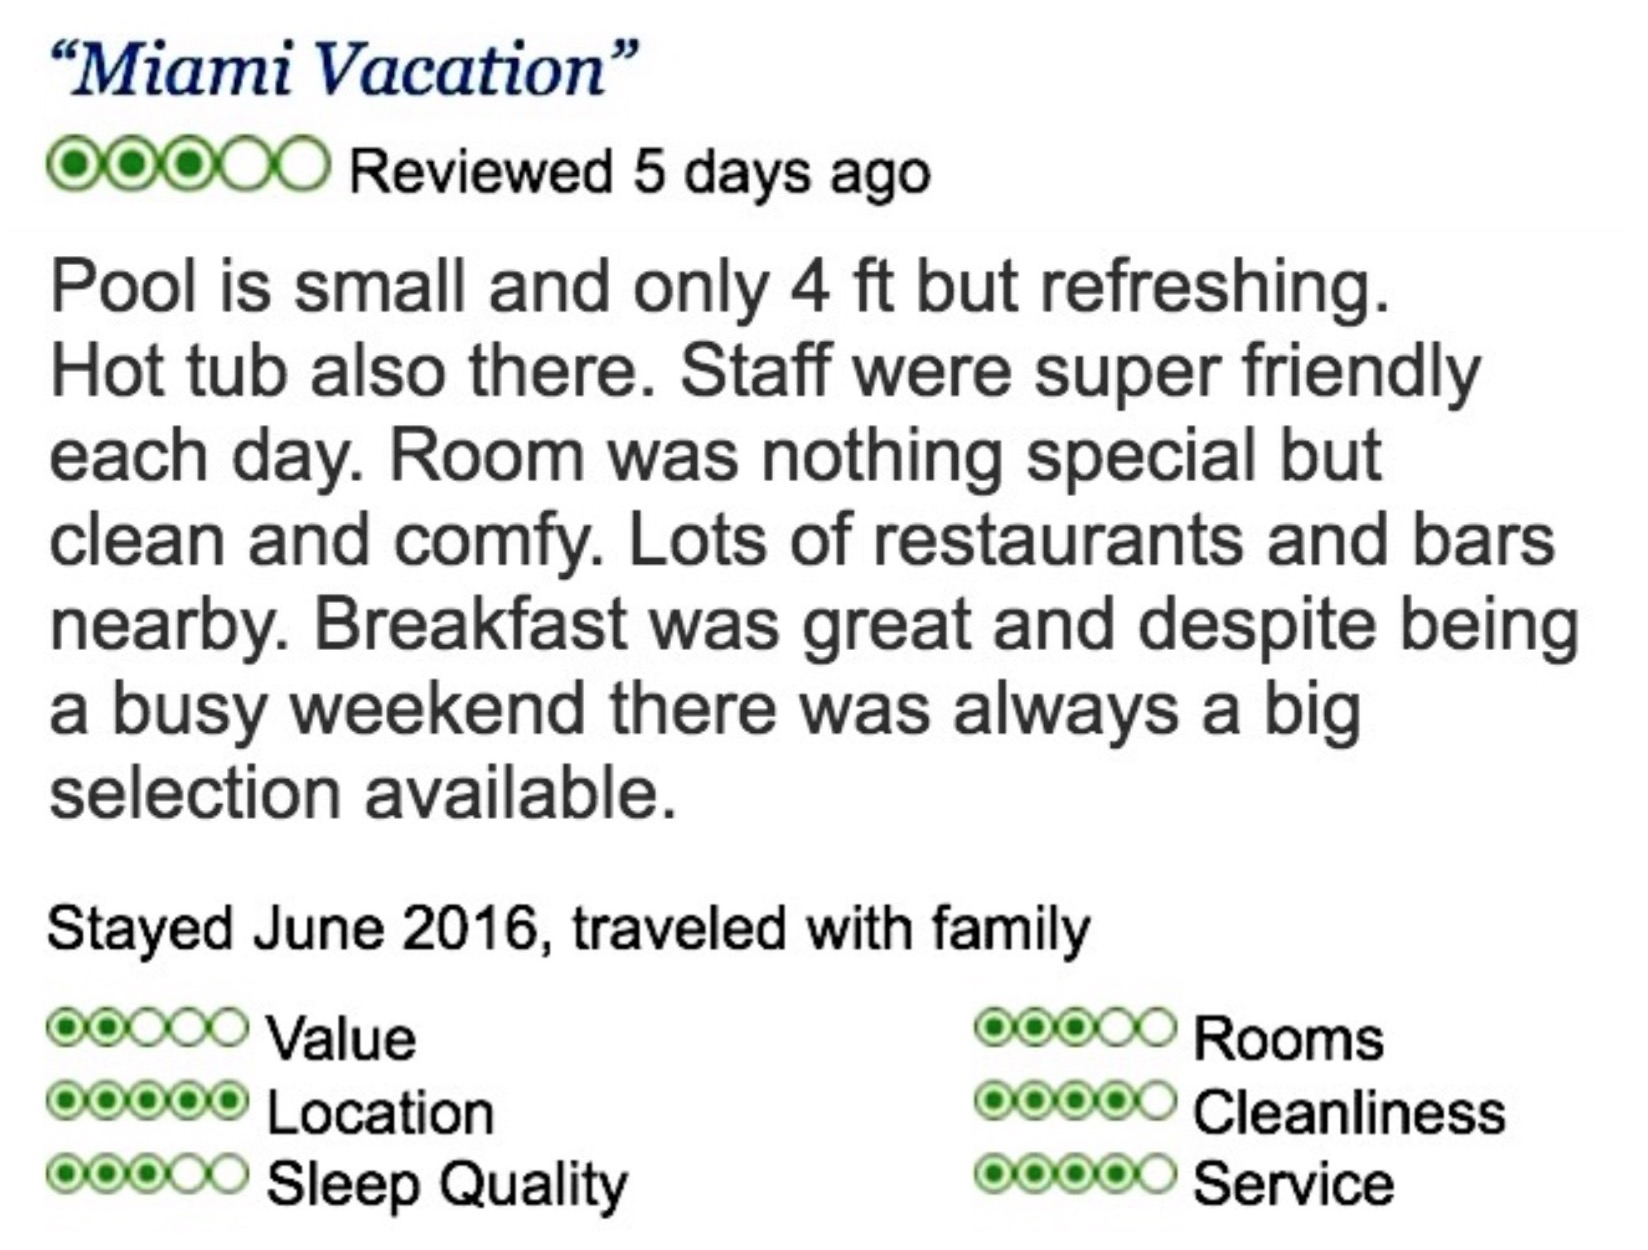
\includegraphics[width=0.6\columnwidth]{figures/tripadvisor}
%	\caption{An example user review about a hotel on TripAdvisor. 
%		The grades are organized by different prominent review aspects: \textit{value}, \textit{rooms}, etc. }
%	\label{fig:tripadvisor}
%%	\vspace{-10pt}
%\end{figure}                                
%2) automatically mined product-specific phrase 
%sets~
%We discuss these two types in the following two paragraphs.
% such as those shown
%about a specific car model in \figref{fig:cars.com}, a snapshot from Cars.com. 
%Aspect-based review summarization is commonly seen on websites 
%like TripAdvisor and Cars.com. 

%Aspect-based reviews have several advantages compared to the more traditional 
%style of online reviews that consists of a short passage and an overall rating. 
%\begin{figure}[th]
%\centering
%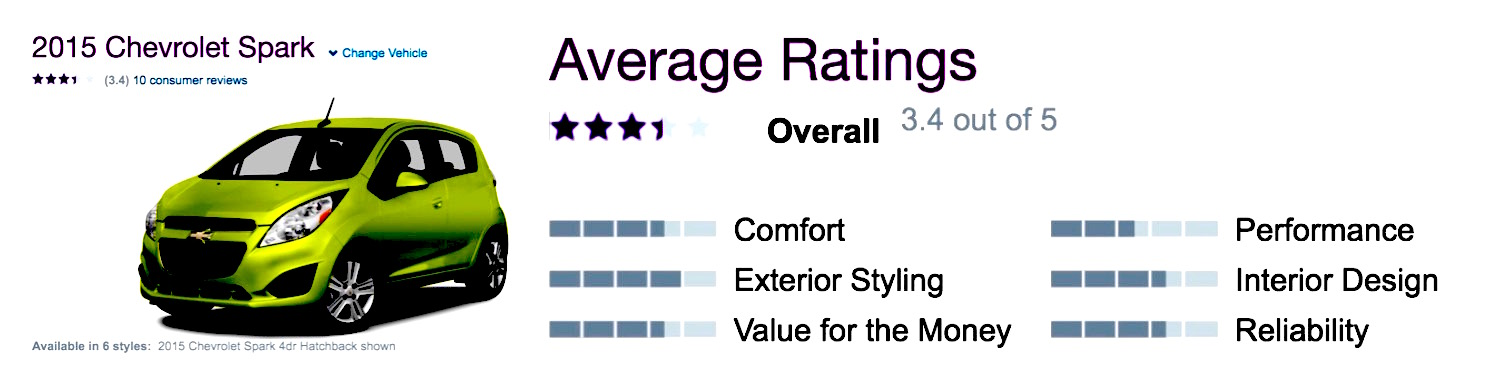
\includegraphics[width=1.0\columnwidth]{figures/cars}
%\caption{Review summarization from Cars.com.}
%\label{fig:cars.com}
%\end{figure}

Existing approaches for producing such prominent aspect terms have been
largely manual work~\cite{poria2014rule,qiu2011opinion}. This is feasible for web services that only 
sell (or review) a small number of  product types of the same domain. 
For example, TripAdvisor.com only features travel-related products, 
and Cars.com only reviews automobiles, so that human annotators can provide 
appropriate aspect terms for customers based on their domain knowledge.  
While it is true that the human knowledge is useful
in characterizing a product type,
%and the desired number of {\em prominent aspect terms} are indeed small enough for human to manually choose them.
such manual approach does not scale well for 
general-purpose e-commerce platforms, such as Amazon, eBay,  
or Yelp, which feature too many product types, 
not to mention that new product and service types are emerging 
everyday.  
In these cases, manually selecting and pre-defining 
aspect terms for each type is too costly and even impractical.
%Therefore, human labor would be too expensive and impractical to attack this task 
%and it can also be difficult for human to predefine aspect terms for 
%some emerging products. 

Moreover, the key aspects of a product type may also change over time. 
For example, in the past, people care more about the screen 
size and signal intensity when reviewing cell phones. 
These aspects are not so much of an issue in present days. 
People instead focus on battery life and processing speed, etc.
Therefore, there is a growing need to automatically extract prominent 
aspects from user reviews.

%\BL{better have an example of emerging product}

%
%Manual selection of aspects 
%certainly cannot scale to such large number of
%product types. 
%These platforms instead turn to automatic review 
%summarization, mined from the user review texts. 

A related but different task is \textit{aspect-based opinion 
mining}~\cite{su2008hidden,zeng2013classification}. 
Here techniques have been developed to automatically mine
product-specific ``opinion phrases'' such as those shown in 
\figref{fig:phrases}.
In this example, the most frequently mentioned opinion phrases
about a phone model along with the mention frequency
are displayed. 
Their goal is to get the {\em fine-grained} opinion summary on
possibly overlapping aspects of a particular product.
For example, ``good looks'' and ``beautiful screen'' both comments
on the ``appearance'' aspect of the phone. However, these aspects
are implicit and can't be used in aspect-based review summarization
directly. The main disadvantage of these opinion phrases is that
their aspects differ from product to product, making it difficult to
compare the product side by side. 

\begin{figure}[th]
	\centering
	\begin{minipage}{0.48\textwidth}
		\centering
		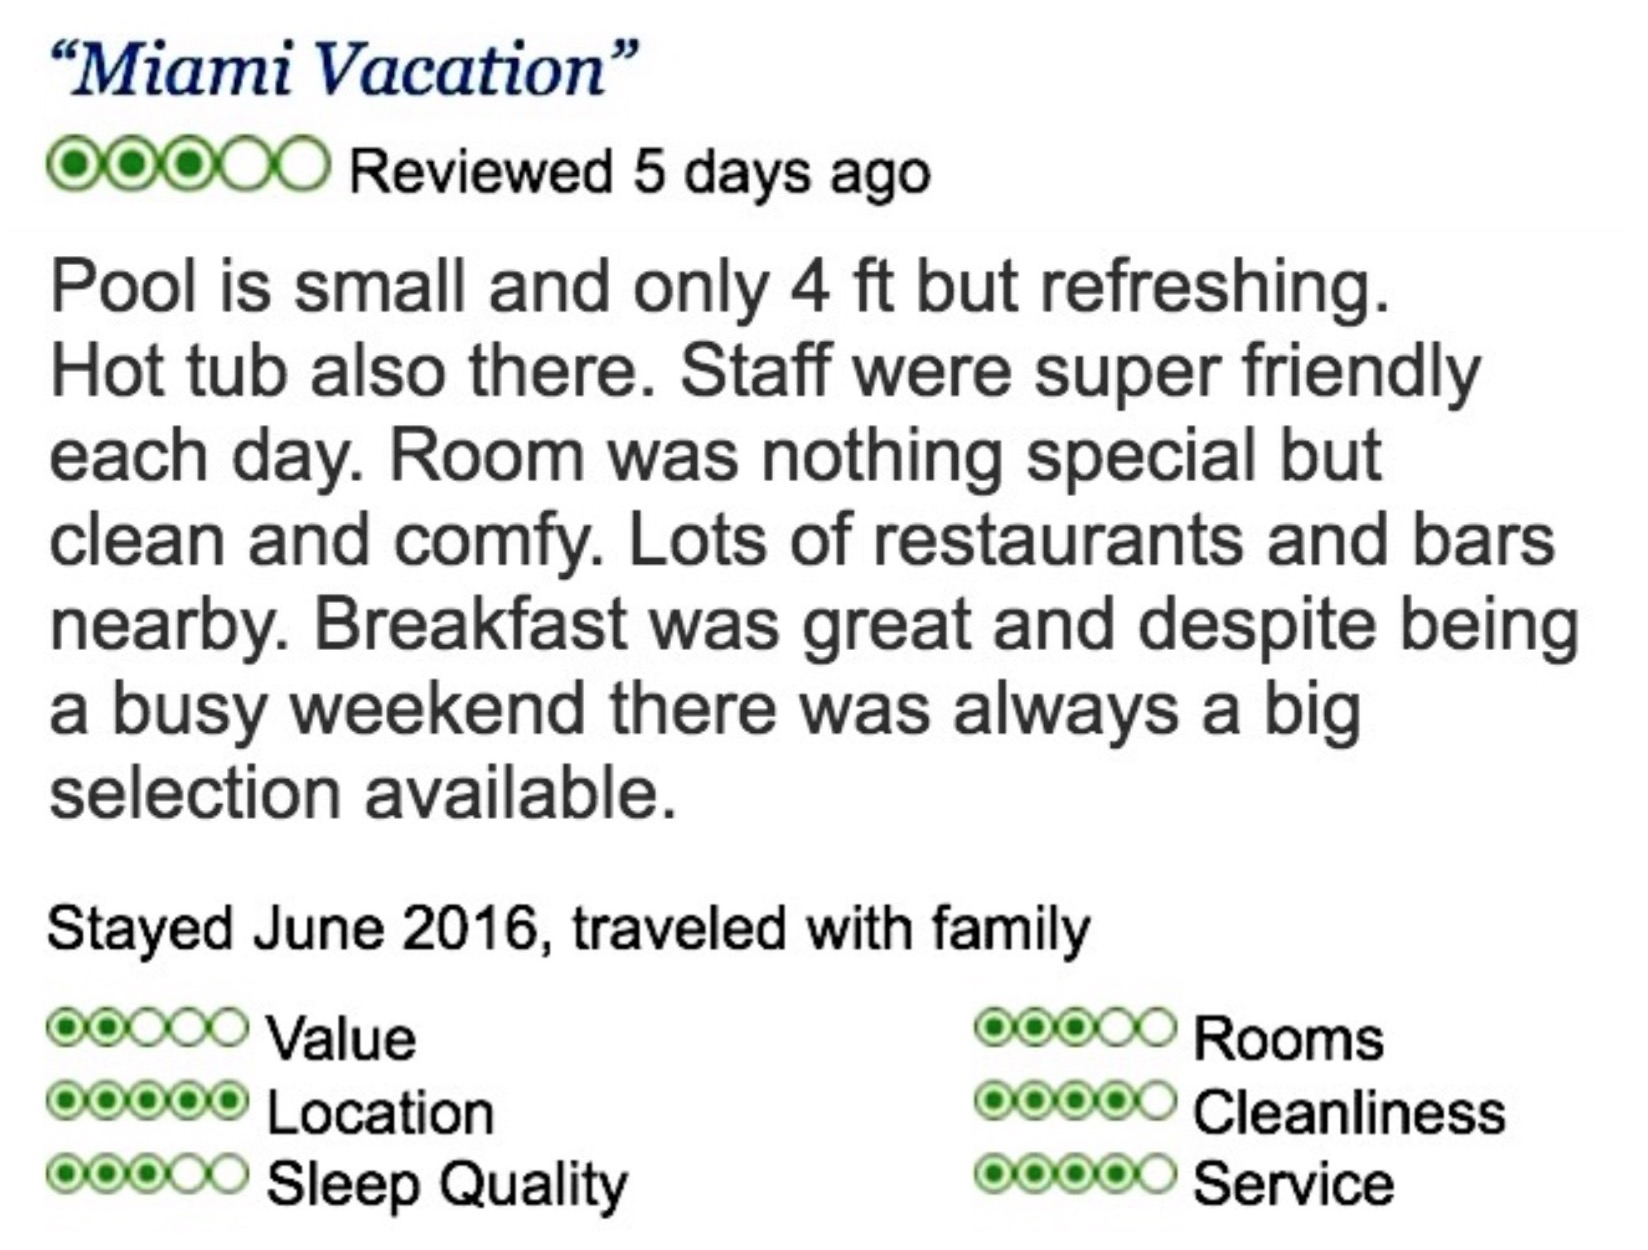
\includegraphics[width=0.7\columnwidth]{figures/tripadvisor}
		\caption{An example user review about a hotel on TripAdvisor. 
			The grades are organized by different prominent review aspects: \textit{value}, \textit{rooms}, etc. }
		\label{fig:tripadvisor}
	\end{minipage}\hfill
	\begin{minipage}{0.48\textwidth}
		\centering
	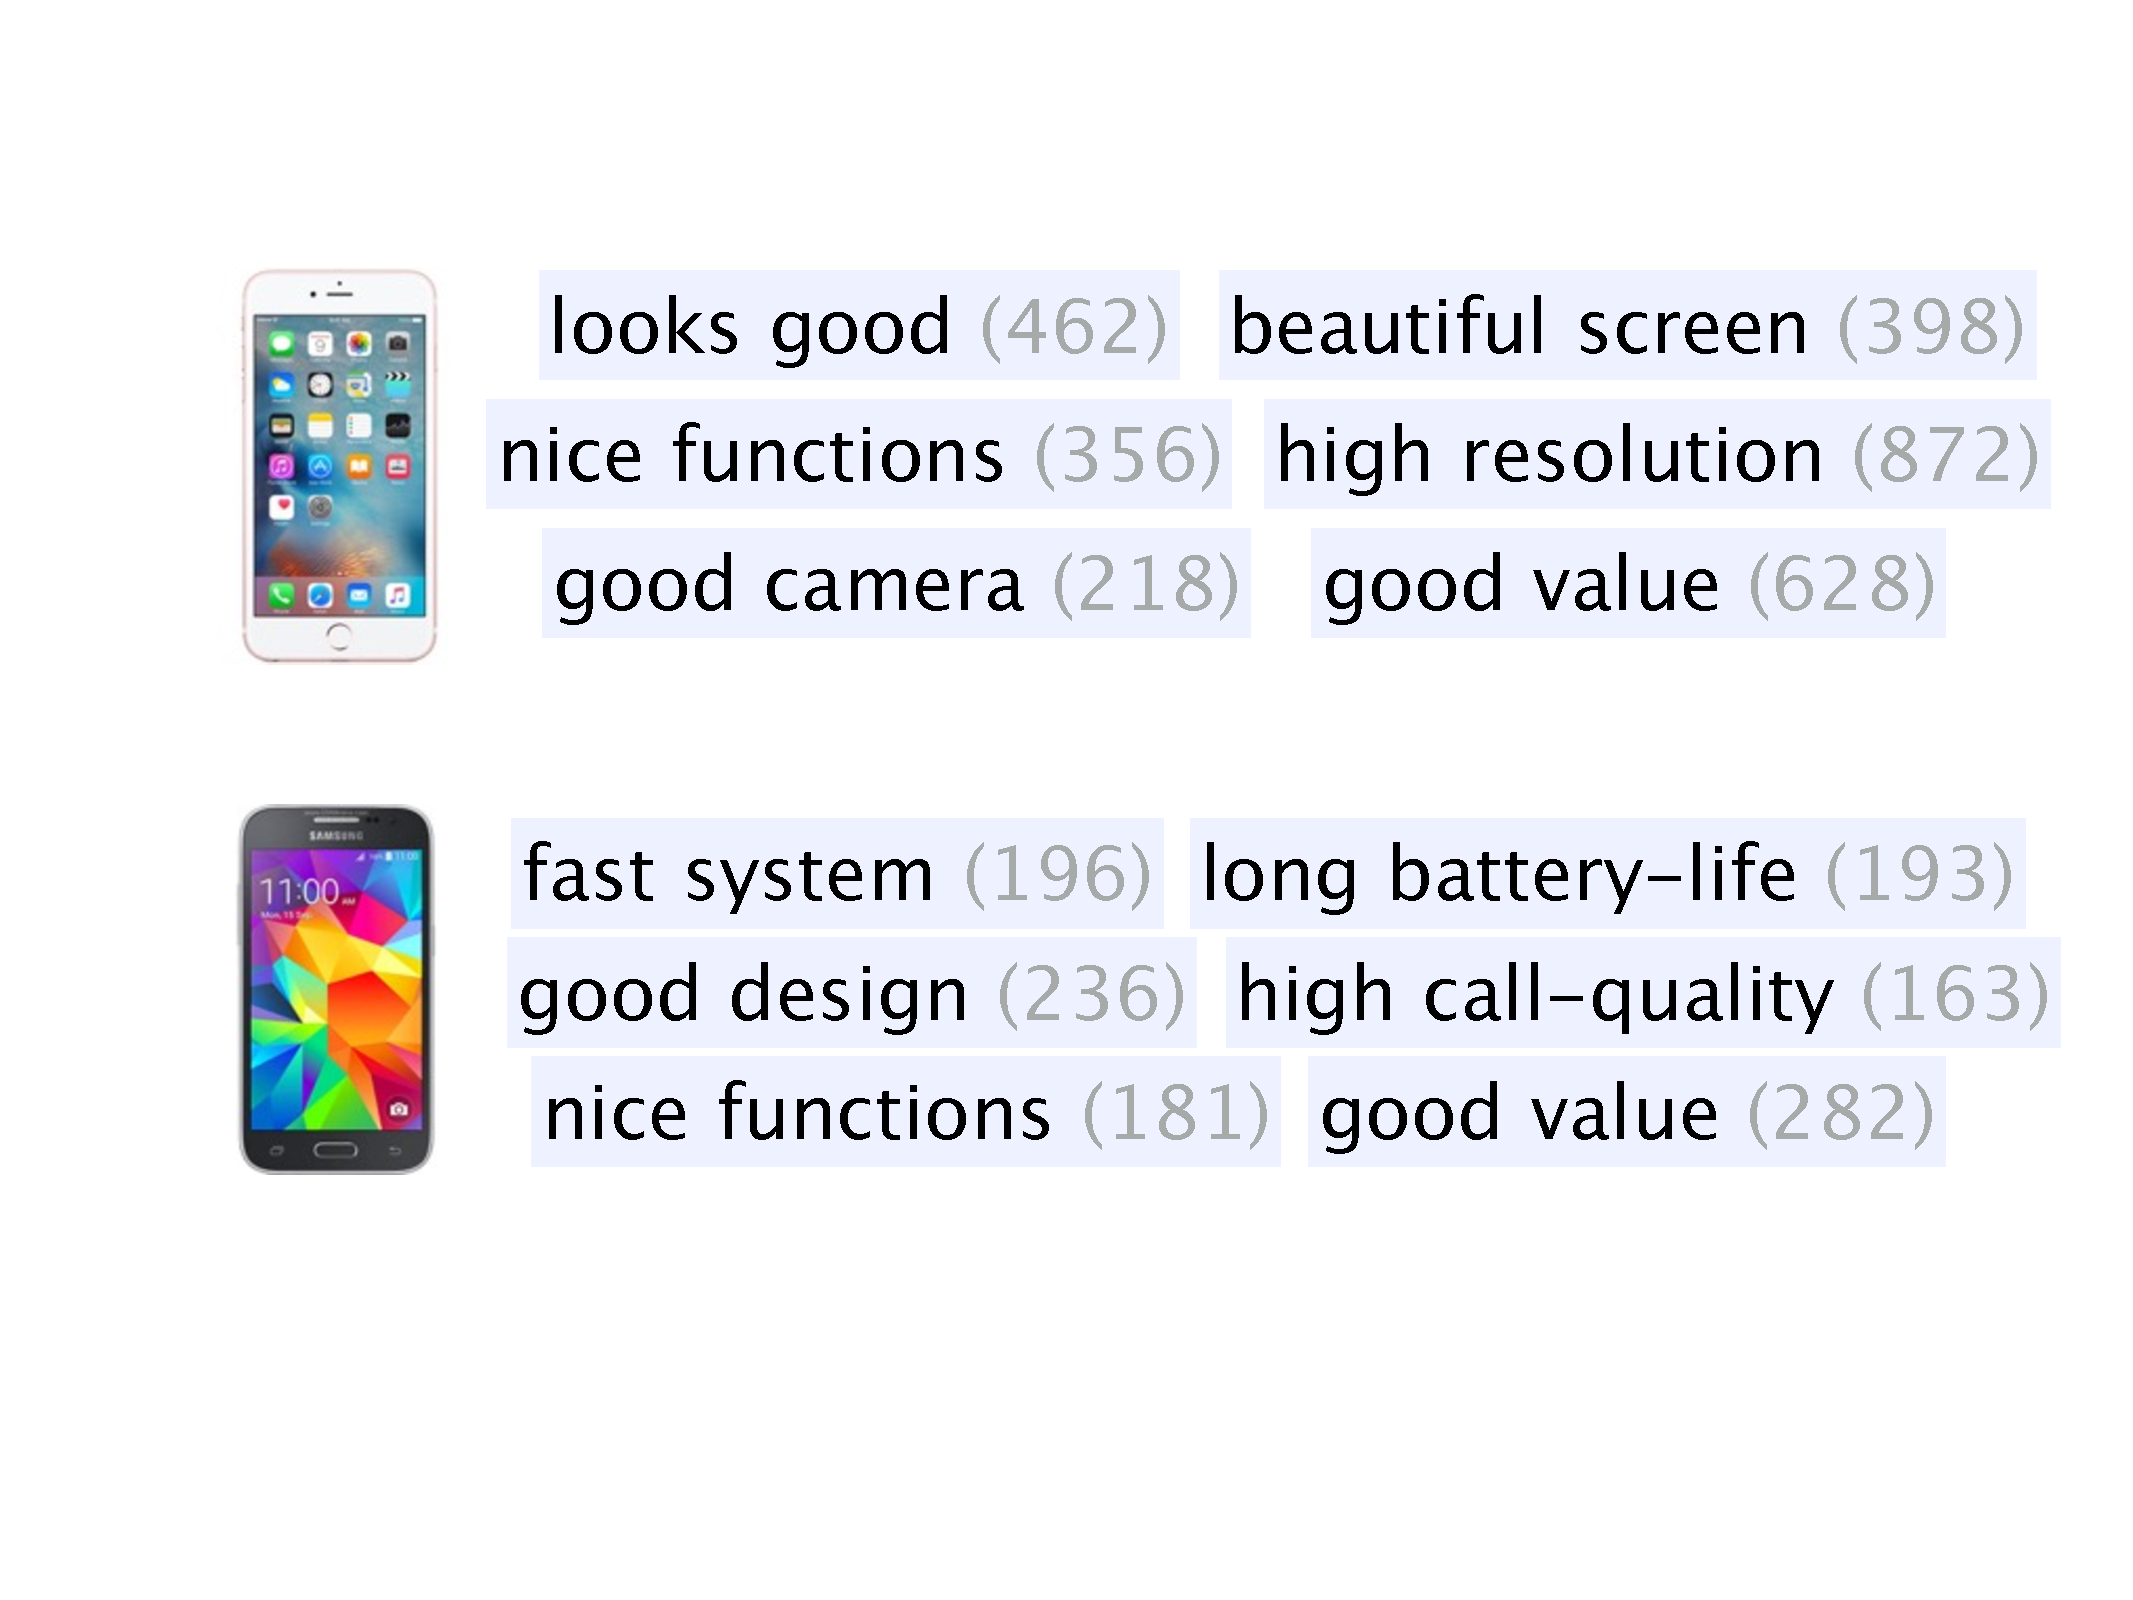
\includegraphics[width=0.9\columnwidth]{figures/phrases}
	\caption{Automatic review summarization for two mobile phones 
		on an e-commerce website}
	\label{fig:phrases}
\end{minipage}
\end{figure}

%There are two set of automatically mined phrases for two 
%different phone models respectively, along with the number 
%of their occurrences
%in the reviews.  
%Such terms are not suitable for aspect-based review
%summarization because: 
%\begin{enumerate}
%	\item aspect phrases for different products of the same type 
%are often different, making it difficult to 
%compare them directly; 
%	\item  emotional terms in the aspect phrases can hinder potential customers to assess products efficiently from different prominent angels.  
%\end{enumerate} 
%
%\vspace{10pt}


%3) this method can only apply on 
% user cannot choose to express them differently.

%The aspects of a product are supposed to capture the most important features 
%and cover all the facets of the product. The products of the same category 
%share the same set of aspects, however the aspects can be very different 
%across categories. It takes both common knowledge and personal experience 
%with the product to decide which are the appropriate aspects. 
%The websites that can provide aspect-based rating system basically 
%all share a common feature, that is they each focuses on only one or 
%a small range of products. For example TripAdvisor focuses on hotels and 
%Cars.com focuese on cars. The set of aspects is what the consumers base 
%on to compare different products, thus they must be carefully chosen 
%to cover all the facest of the product. Moreoever, at the end of the day 
%the aspects is designed to serve the consumers, especially potential consumers, 
%so they need to reflect what the consumers care about the product. 
%Ideally, the aspects should be decided with user reviews taken into 
%consideration. For a small range of products, the website owner or 
%the retailer may manual designate the set of aspects, 
%however this is intractable for websites like Amazon and TaoBao, 
%which host basically all kinds of products available on the market, 
%and websites like Yelp on which users review thousands of different services. 
%
%Motivated by this observation, we are in need for methods that automatically 
%generate review summarizations. 

The goal of this paper is to develop an unsupervised framework 
for automatically extracting $K$ most prominent, non-overlapping 
review aspects for a given type of product from user review texts.  
%The formulation of aspects extraction, 
%which is extracting words from a set of documents, 
%is similar to topic modeling where aspects can be seen as topics. 
%While the task seems to be similar with topic modeling on the a set of review documents,
Developing such an unsupervised framework is challenging for 
the following reasons: 
\begin{itemize}
    \item 
	The extracted prominent aspects not only need to cover as many customer concerns as possible but also have little semantic overlap. 
    \item The expression of user opinions is highly versatile: 
aspect terms can be expressed either explicitly or implicitly. For example,
the mention of ``pocket'' implies the aspect ``size''.
% \KZ{Do we have example of this?}
    \item Product reviews are information rich. A short piece of comments 
may target multiple aspects, so topics transit quickly from sentence 
to sentence. 
\end{itemize}

Most previous unsupervised approaches for the prominent 
aspect extraction task are variants of topic modeling 
techniques~\cite{lakkaraju2011exploiting,lin2009joint,wang2011latent}.
The main problem of such approaches 
is that they typically use only word frequency and co-occurrence information, 
and thus degrade when extracting aspects from sentences that appear
different on the surface but are actually discuss similar aspects. 
%\BL{Jessie please describe our framework briefly here, using similar words in the following sections} 

Given all review text about a certain product type, our framework, ExtRA,
extract most prominent aspect terms in four main steps: 
first it extracts potential aspect terms from text corpus by lexico-syntactic 
analysis; then it associates
the terms to synsets in WordNet and induce a subgraph that connect these
terms together; after that it ranks the aspect terms by a personalized page rank
algorithm on the sub-graph; and finally picks the top $K$ non-overlapping 
terms using the subsumption relation in the subgraph. 

%substitutes mentions of noun words and high quality phrases to 
%Wikipedia concepts by leveraging Wikipedia redirected links.
%Such preprocessing step can aggregate synonyms with different mentions together. For example, we substitute {\em front desk} , {\em administrative assistant}, {\em reception desk} mentions to {\em receptionist} concept in wikipedia. 
%Then, ExtRA clusters 
%all the review sentences into several \textit{sentence cluster}s.  
%Furthermore, within each sentence cluster, 
%we perform \textit{topic modeling} to obtain potential aspect topics.
%We further cluster all the potential topics across sentence clusters to 
%produce the final refined \textit{topic cluster}s, based on our designed vectorial representation for word distributions (\textit{AspVec}).
%%For refinei topic clusters and ranking candidate aspect terms respectively, we propose two ranking metrics, which help us 
%Aspect clusters are then properly represented as vectors (AspVec) in a shared space with aspect terms. 
%By encoding the topic clusters into vectorial representations (),
%Then, ExtRA can extract the most prominent aspect terms and phrases 
%based on similarity computation.
%\ZY{In order to extract $K$ best aspects, we carefully design a ranking mechanism including two ranking metrics respectively for pruning aspect clusters and ranking candidate aspect terms, }
%in which we represent aspect clusters with vectors (AspVec) in a shared space with aspect terms.
%with aspect candidates benefiting from our ranking mechanism. 
  
The main contributions in this paper are as follows:
\begin{enumerate}
    \item We propose a novel unsupervised framework for extracting 
prominent aspects from customer review corpora (\secref{sec:method}).
    \item Extensive experiments show that our framework is effective and 
outperforms the state-of-the-art methods by a substantial margin (\secref{sec:experiments}).
    \item We release an open-source implementation of the framework 
    and the evaluation dataset for future work in this research area.
%\item We demonstrate a downstream application of our ExtRA framework, which can benefit existing aspect-based review analysis systems.
%\item We will publish our aspects taxonomy for further research purpose.
%\item We also built a demo website\footnote{Our demo website is available at \url{http://anonymized.due.to.blind.review}} for visualizing the mined review aspects and their potential applications.
\end{enumerate}

%The rest of this paper are organized as follows.
%In \secref{sec:method}, we introduce the ExtRA framework in detail.
%In \secref{sec:experiments} we evaluate the proposed framework on a dataset consisting multiple domains. A downstream application of ExtRA is demonstrated in~\secref{sec:demo}.
%% demonstrate 
%%the effectiveness of our model against other approaches 
%%and show how the extracted aspects can be used
%%to construct a complete review summarization. 
%Finally, in~\secref{sec:related}, we discuss
%and compare our work with previous research related to aspect-based review analysis.
%
